From the practicioner's perspective, we are interested in thinking about the "metaphysical unit" of scientific practice on a finer scale than allowed by Feyerabend's concept of a tradition. If we take the practice of molecular biology to be about generating explanations for biological phenomena in terms of macromolecules, we want to know enough about the structure of these explanations to allow us to compare them. While we all already know that we are looking for the "underlying molecular mechanisms" of (usually) cellular phenomena, it is not always clear how we might go beyond intuitive preferences for one proposed mechanism or another in, say, deciding what assay to perform next. We may reason in terms of plausibility or agreement with evidence, but we rarely do so formally\footnote{.}


\subsection {Classical and Molecular Genetics: Shared Traditions, Plural Methodologies}
\label{PS}
To bring the implications of Feyerabend's views into some familiar relief, let us briefly examine a case from the field: the ``molecularisation" of zebrafish genetic experimentation. Because the zebrafish genome took some time to be released in reliable revision, the use of the Mendel/Morgan ``classical genetic tradition" (CGT) was widespread in mapping experiments before this. One might locate an allele of interest by recombination experiments, mapping its position in (by now unfamiliar) units of centimorgans to reflective relative recombination frequency between loci. This is, of course, increasingly unusual, as the practices of the Watson/Crick ``molecular genetic tradition" (MGT) are more and more accessible due to the previously unavailable genomic data\footnote{It can be an edifying experience to ask a student to ``convert" between CGT units like centimorgans and MGT units like megabases. At the very least, the cognitive discomfort produced will tend to reveal a problem in the question's assumptions to the student. At best, one can gain a practical understanding of how scientists make sense of and experience ``switching" between different traditional explanatory frames.}. The zebrafish geneticist now has access to two traditions to perform their work, and will make recourse to either as they assess circumstances warrant (without any reference to an explicit external rule about which tradition should supercede the other in particular cirucmstances). For instance, if I am planning to cross two fish that are heterozygous at some allele, I will use typical CGT assumptions to calculate the expected number of various offspring genotypes. Even if I was able to offer a reasonable description, in molecular terms, of zebrafish meiosis, recombination, fertilisation, and so on, I would never choose to do so- an MGT explanation is unnecessary where Mendel's laws suffice, and will begin to lack explanatory power the moment I apply it to another species, unlike the Mendellian CGT framework.

One might object that the claims of the CGT tradition ``reduce" in some meaningful way to the MGT tradition, or ``cover" for it, so that CGT theories are in fact just abstractions of MGT theories. In other words, the fact that MGT claims are not useful and lack explanatory power in some areas does not change the fact that MGT \textit{could} provide good theoretical explanations for all of the claims of CGT. As Kitcher shows, this is not correct\footnote{Kenneth Schaffner later insisted that Kitcher was wrong, and that CGT theories are reducible to MGT theories, because the MGT theories establish direct linkages between DNA sequences and proteins, and thus are formally equivalent to the classical concepts of genes and phenotypes \cite{Schaffner1993}. This now seems obviously mistaken on at least 2 counts: (1) there is no stable molecular entity implicated by ``the gene": its local context in terms of primary sequence (promoters etc.), and tertiary arrangement in a nuclear ``transcription factory", all contribute to the complexity of the causal locus involved in transcription alone, and (2) there are very few phenotypes of interest that are caused by stable, uncomplicated interactions between DNA and protein such that classical genetic phenotypes reduce cleanly or usefully to descriptions solely in terms of macromolecules. Moreover, this does not address Kitcher's point: there \textit{are} phenotypic traits which are \textit{not} describable in terms of their protein constituents, and that there \textit{are} higher-level processes which may be generated by any number of configurations of molecular consituents and are thus better understood as types of processes and not as specified molecular systems.}. The CGT description of the \textit{process} of meiosis as a particular type in which ``paired entities (i.e. chromosomes) are separated by force so that one member of each pair is assigned to a descendent entity"\cite[p. 349]{Kitcher1984} (which Kitcher calls a PS-process), is not describable solely in terms of the molecules participating in the process. Because a PS-process like meiosis can be realised in any number of ways at a molecular level, PS-processes cannot be accounted for in a general way by MGT theories. The manner in which different traditions frequently address different levels of biological organisation in similar non-interchangeable ways is discussed further below.

We can extend this example to see that the typical biologist has access to a great plurality of methodological traditions. Biologists are intuitively used to ``translating" between traditions and to switching freely between them when translations are cumbersome or useless. Where there are no deep conflicts between the implict aspects of these traditions, no counterinductive process occurs. That is, we do not ``refute" CGT with MGT in the same way the Copernican Revolution ``refuted" Aristotlean geostatic theory because MGT rarely makes the structure of CGT seem untenable to us; an attempt to replace CGT with MGT would surely be quixotic. We simply appropriate the methodology of the tradition which is most appropriate for the problem at hand.

\subsection{Sense of ``Tradition" in this study}

Thomas Kuhn was soundly criticised for the vague sense in which he used the term ``paradigm"\cite[p.206]{Schaffner1993}, which left him unable to offer coherent explanations. Feyerabend was far more precise, but, as a philosopher rather than a practitioner, never had need (or desire) to guide a scientific project from within the worldview he developed. Having erected an unassailable proof that no special Method existed, and that subscribing to one would have prevented the central Galilean vignette of naive philosophy of science's core Enlightenment self-narrative, he effectively retired\footnote{Feyerabend's chilly reception and subsequent exile is difficult to understand in retrospect, as the basic framework of his argument is now generally understood to be correct in some sense or another. Whether one ascribes the initial poor reaction to his combative personality or flamboyant political statements, his ideas are by now pervasive, even normative. The appearance of ``post-colonial" biological studies would have been very unlikely in the Popperian scientific world of the 1960s. Curiously, the Feyerabendian molecular biological traditionalist will note that this may actually constitute an intra-traditional ``colonial" venture on the part of critical theorists and continental philosophers.}.

When Feyerabend wrote of ``scientific traditions", he meant scientific practice in its broadest possible sense, a social practice with ``historico-physiological character". That is, scientific theories are conditioned by the historical moment, and by the involvement of the observer and their social, cognitive, and biological baggage in the phenomenon under study. For the purposes of making Feyerabend's arguments against the existence or advisability of a mono-Method, this was entirely adequate, but I intend only to deal with a limited subset of these materials. The ``Stem Cell Biological Tradition" defined below, in its full Feyerabendian sense, includes rumours circulated at stem cell conferences, methodological tips and tricks passed on by observation of careful practice (that could never be learned from any protocol), the commercial aspirations of particular academics, and so forth, in addition to all of the ``properly scientific" materials implicated by all of the publications that have ever used the ``stem cell" concept or a recognisable homologue. While my use of the term acknowledges this broader contextual sense, I will only look at the explicitly documented ``traditional background" of particular, formally advanced explanatory statements or models. The objective here is mainly to account for molecular biological explanations occuring within a ``composite tradition" with diverse, only partially overlapping internal ``subtraditional" currents.

Therefore, in general, I have not intended to draw any hard divisions between subtraditional currents in the molecular biological tradition (MBT). While I have pointed out how MBT explanations may include components drawn from irreducibly separate subtraditions (the irreducible CGT explanation for PS-processes discussed \hyperref[PS]{above}), I have only mentioned the philosophical, methodological, etc. implications of MBT subtraditions where necessary, as the primary concern is the extra-traditional background of the ``systems" modelling approaches encountered in the data chapters. For instance, in the case of the Galton-Watson branching process model, my definition of this as an artefact (one can think of a probability distribution plot figure in a paper) from the Probability Theory Tradition (PTT) means that this is a traditional statistical solution to an early biological lineage model, which stands in for the large-scale behaviour of a simple model of lineage growth and extinction, in a larger MBT mechanistic explanatory framework (the \hyperref[EHJMEx]{MEx}, Mechanistic Explanation).

I have also made reference to the ``Stem Cell Biological Tradition" (SCBT), which is intended to convey the last approximately 6 decades of research practice organised around the stem cell concept\footnote{I include anti-stem cell and stemness theories in this tradition, since they are marginal heresies to a hegemonic orthodoxy and not meaningfully independent.}. The question of the relationship between the MBT and SCBT is not simple. Till and McCulloch were not offering molecular mechanisms for the phenomena they were documenting \cite{McCulloch1960}, and could well have been described as operating in an earlier Cell Biological Tradition (CBT).

 My conception of this relationship is that, generally, SCBT practice has been ``molecularised"; most of the explanations that SCBT practitioners care about are molecular MEx, and the SCBT is therefore a subtradition of the MBT. Nevertheless, the \hyperref[hierarchy]{multilevel} character of all MBT explanations means that SCBT practicioners routinely use CBT concepts where a specified molecular system would be useless or inappropriate. An example is the ubiquitous abstraction of mitotic phenomena as a class of cell behaviour in SCBT explanations (referred to simply as ``mitosis", ``proliferation", ``renewal" etc), rather than making any attempt to specify this central concept in explicitly molecular terms.

 Therefore, in this sense, SCBT practitioners are used to ``slotting in" explanatory components from a variety of traditions in order to offer a broader MEx for some phenomenon (regeneration, repair). We are in this sense classic Feyerabendian ``Epistemological Anarchists", using whatever explanatory frames suit our purposes. This habit has, in the context of the \hyperref[SBE]{SBE}, shifted from predominantly ``intra-" to ``inter-traditional anarchism", with the result that the required level of sophistication required to advance a good molecular MEx has increased steeply.
 
 The SCBT is a particularly notable subtradition of the MBT because of its explicitly therapeutic, and therefore ethical and normative orientation. That is, while the broader developmental biology tradition does not have a unified therapeutic goal, the SCBT is structured by the objective of interacting with stem cell phenomena to medicinal and therapeutic ends. This particularly ethical aspect of the SCBT compels me to make some brief remarks about how my own study's design is be guided by this ethical orientation.

\subsection{Time}
\label{time}
\subsection{Semiosis, Meaning}
\label{semiosis}
\subsection{Emergence, self-organisation}
\label{emergence}
\subsection{Scale Hierarchies, Specification Hierarchies}
\label{hierarchy}
\subsection{Waddington's topological model of development}
\label{Waddington}
\begin{longquote}
C. H. Waddington was one (and almost certainly the
best remembered) of the embryologists who so profited. He
wrote: “During the recent war, engineers attained some fa-
cility in designing machines to carry out tasks which earlier
generations would have considered beyond the capacities of
anything but an intelligent being . . . The ideas suggested
by these self-regulating mechanisms are both very relevant
to biology and rather novel.” 28 Waddington himself worked
in the Operation Research Section of the Royal Air Force
Coastal Command, and it was from his own experience and
from that of his friends in self-steering gunnery that he
learned to draw the analogy which was to become increas-
ingly familiar in the cybernetics of the 1950s and 1960s: “The
behaviours of an automatic pilot, of a target-tracking gun-
sight, or of an embryo, all exhibit the characteristics of an
activity guided by a purpose.” 29 Indeed, it was at this time,
and in this context, that his work on canalization began. 30
In Waddington’s first introduction of the term, he
wrote, “The main thesis is that developmental reactions as
they occur in organization submitted to natural selection,
are, in general, canalized. That is to say, they are adjusted so
as to bring about one definite end result regardless of mi-
nor variations in conditions during the course of the reac-
tion.” In his view, canalization is built into the organism by
natural selection as a consequence of its obvious advan-
tages: “It ensures the production of the normal, that is, op-
timal type in the face of the unavoidable hazards of exis-
tence.” 31 Canalization was a term Waddington had borrowed
from his reading of Alfred North Whitehead, and the con-
cept clearly accorded with much of his own prewar thinking
about “epigenetic landscapes.” 32 But it was only after the
war that he began to envision the possibility of a theoretical
account of such characteristic features of biological organi-
zation. An explanation of “developmental canalization,” he
wrote, requires supplementing conventional gene theory
with an “epigenetic theory”—one in which discrete and sepa-
rate entities of classical genetics would be displaced by col-
lections of genes which could ‘lock in’ development through
their interactions.” 33 In other words, an account of develop-
mental stability needs to be sought in the complex system
of reactions that make up the developmental process.
The search for quantitative models displaying such be-
havior underlay much of Waddington’s theoretical efforts
well into the 1970s. However, he soon concluded that the
particular models developed by Ross Ashby and other cyber-
neticians on self-organizing systems were not really appro-
priate to biological development. Instead, he concentrated
on feedback models of cross-reacting systems of metabolic
reactions. Yet he did not have a great deal of success with
these models. Indeed, it is not his theoretical work but the
experimental work from his laboratory in the 1940s and ’50s
that now, with the benefit of hindsight, attracts the most in-
terest.
\cite[p.117-119]{Keller2000}
\end{longquote}

\begin{figure}
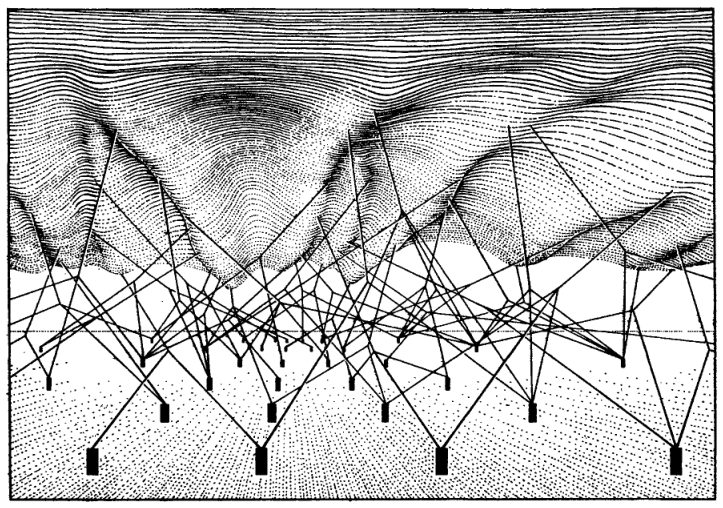
\includegraphics[scale=.5]{Waddington}
\centering
\caption{The complex system of interactions underlying the epigenetic landscape, excerpted from \cite{Waddington1957}.
The pegs in the ground represent genes; the strings leading from
them the chemical tendencies which the genes produce. The
modelling of the epigenetic landscape, which slopes down from
above one's head towards the distance, is controlled by the pull
of these numerous guy-ropes which are ultimately anchored to
the genes.}
\label{fig:Waddington}
\end{figure}